% -*- mode: noweb; noweb-default-code-mode: R-mode; -*-
\documentclass[a4paper]{article}

\usepackage{a4wide}
\usepackage{subfigure}
\renewcommand{\familydefault}{\sfdefault}
% \usepackage{fancyhdr}
% \pagestyle{fancy}



\title{PIL Response Score for A/B at Price 0.56}
\author{Lily Wang}







\usepackage{Sweave}
\begin{document}
\maketitle
\setkeys{Gin}{width=0.5\textwidth}


\section{Introduction}

The overall response rate is 13.56\%, 
and there are in total 4026 records, out of which 546 
records with response = 1, and 3480 records with response = 0. 


\section{Model Description}
\subsection{Logistical Regression Output}
% latex table generated in R 2.11.1 by xtable 1.5-6 package
% Mon Mar 14 13:36:18 2011
\begin{table}[ht]
\begin{center}
\begin{tabular}{rrrrr}
  \hline
 & Estimate & Std. Error & z value & Pr($>$$|$z$|$) \\ 
  \hline
(Intercept) & -0.0092 & 0.2070 & -0.04 & 0.9644 \\ 
  TOT\_INT\_FEE\_mth6\_d2 & 0.4771 & 0.2126 & 2.24 & 0.0248 \\ 
  no\_ln\_matured\_d2 & 0.5315 & 0.1438 & 3.70 & 0.0002 \\ 
   \hline
\end{tabular}
\end{center}
\end{table}
\subsection{Characteristic Table}
% latex table generated in R 2.11.1 by xtable 1.5-6 package
% Mon Mar 14 13:36:18 2011
\begin{table}[ht]
\begin{center}
\begin{tabular}{rrrrrrrl}
  \hline
 & coeff & score & total.pct & Resp = 1 & Resp = 0 & odds & desc \\ 
  \hline
(Intercept) & -0.01 & -0.27 & 100.00 & 546 & 3480 & 0.16 & say sth 
 about your variable \\ 
  TOT\_INT\_FEE\_mth6\_d2 & 0.48 & 13.77 & 82.56 & 521 & 2803 & 0.19 & say sth 
 about your variable \\ 
  no\_ln\_matured\_d2 & 0.53 & 15.34 & 8.49 & 97 & 245 & 0.40 & say sth 
 about your variable \\ 
   \hline
\end{tabular}
\end{center}
\end{table}
\section{Score Performance}
KS:  35.98\% \\
Socre distribution:
\begin{center}
% latex table generated in R 2.11.1 by xtable 1.5-6 package
% Mon Mar 14 13:36:18 2011
\begin{table}[ht]
\begin{center}
\begin{tabular}{rrrrrrr}
  \hline
 & Min. & 1st Qu. & Median & Mean & 3rd Qu. & Max. \\ 
  \hline
overall & 491 & 522 & 545 & 548 & 570 & 657 \\ 
  Resp = 0 & 491 & 520 & 541 & 544 & 564 & 657 \\ 
  Resp = 1 & 496 & 550 & 572 & 572 & 594 & 655 \\ 
   \hline
\end{tabular}
\end{center}
\end{table}\end{center}


\begin{figure}[!ht]
\centering
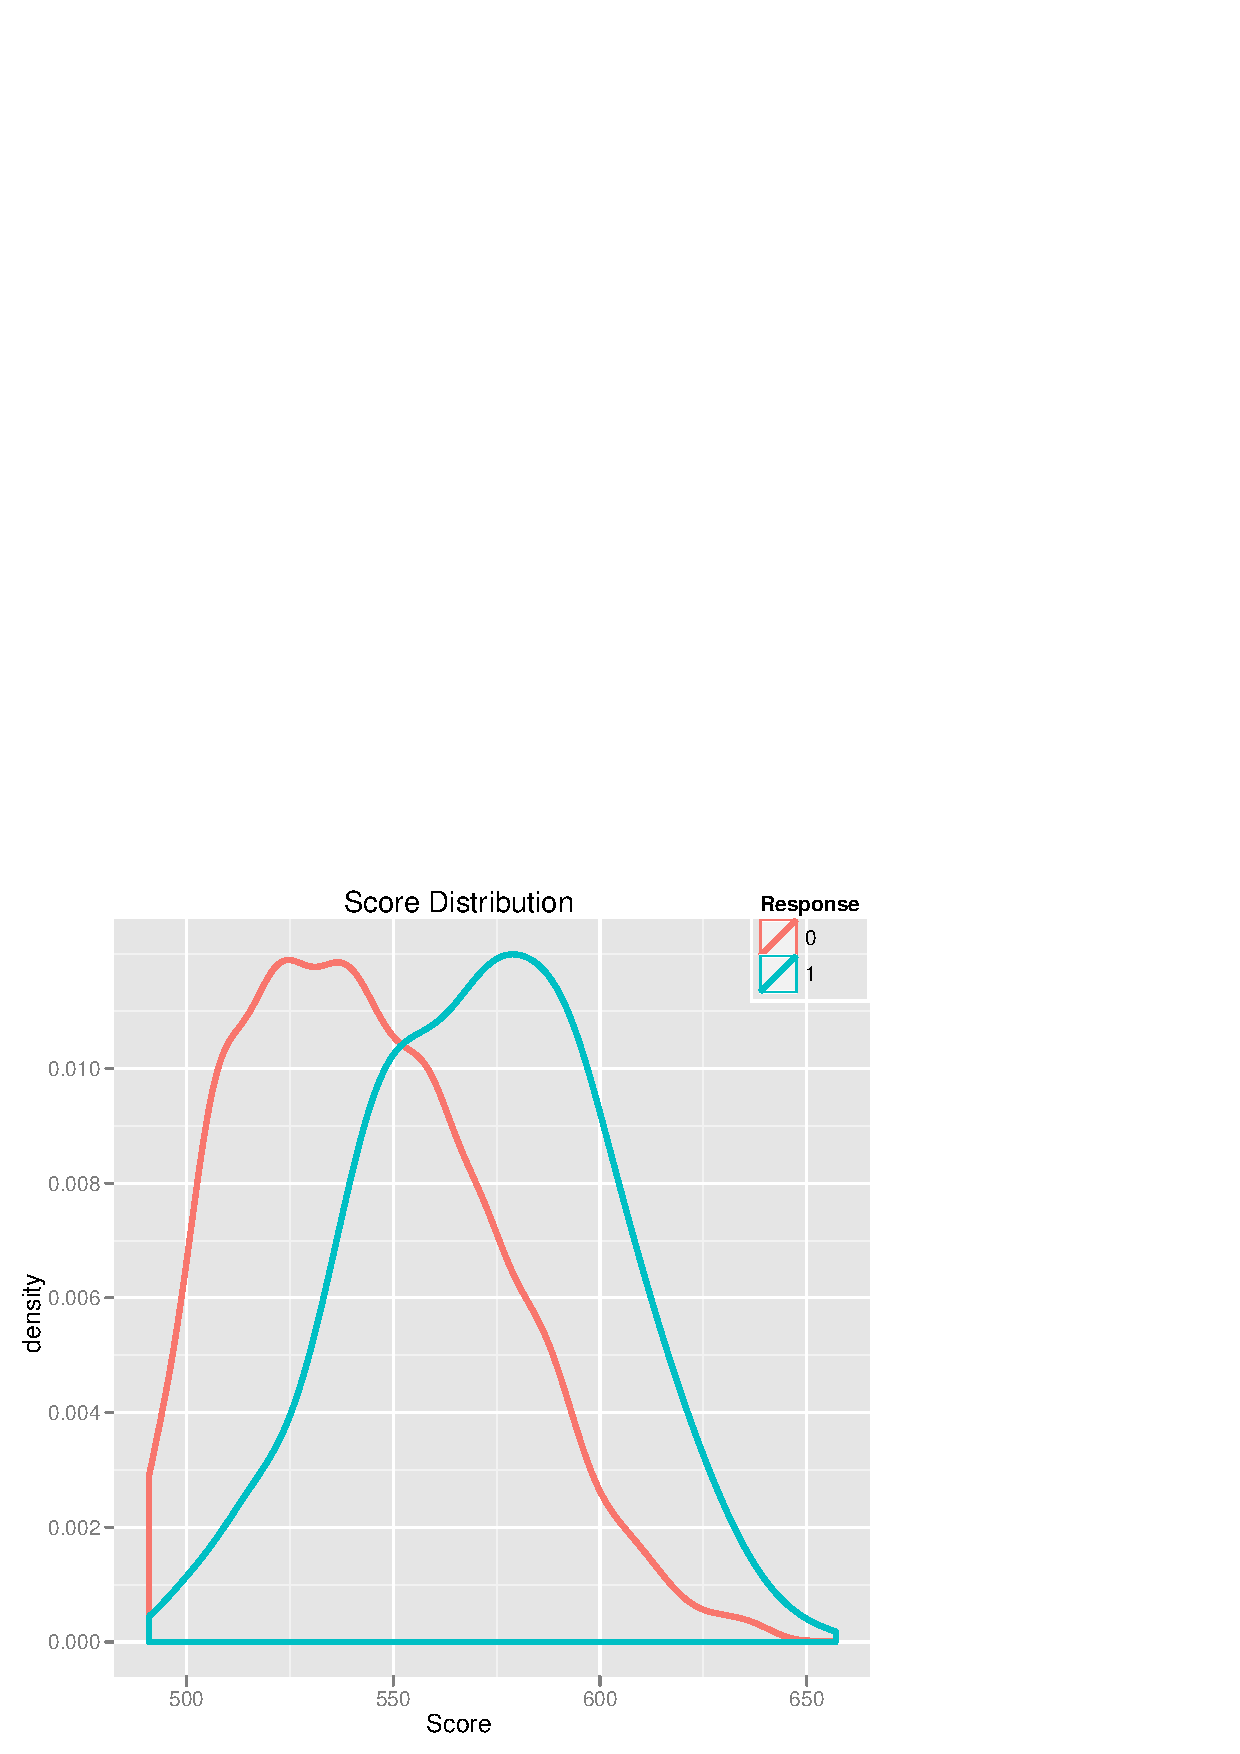
\includegraphics{score-by-y}
\caption{Score Distribution by Response}
\end{figure}


\subsection{KS table and plot by score band}  
% \begin{center}
% <<>>=
% print(score.table[,1:7])
% @
% \end{center}
% latex table generated in R 2.11.1 by xtable 1.5-6 package
% Mon Mar 14 13:36:22 2011
\begin{table}[ht]
\begin{center}
\begin{tabular}{rrrrrrrr}
  \hline
 & Y=0 & Y=1 & Total & \%(Y=0) & \%(Y=1) & \%Total & Act.RR \\ 
  \hline
[-Inf,500] & 174 & 5 & 179 & 5.00 & 0.92 & 4.45 & 0.03 \\ 
  (500,515] & 506 & 14 & 520 & 14.54 & 2.56 & 12.92 & 0.03 \\ 
  (515,530] & 638 & 30 & 668 & 18.33 & 5.49 & 16.59 & 0.04 \\ 
  (530,545] & 615 & 60 & 675 & 17.67 & 10.99 & 16.77 & 0.09 \\ 
  (545,560] & 550 & 86 & 636 & 15.80 & 15.75 & 15.80 & 0.14 \\ 
  (560,575] & 432 & 96 & 528 & 12.41 & 17.58 & 13.11 & 0.18 \\ 
  (575,590] & 313 & 98 & 411 & 8.99 & 17.95 & 10.21 & 0.24 \\ 
  (590, Inf] & 252 & 157 & 409 & 7.24 & 28.75 & 10.16 & 0.38 \\ 
   \hline
\end{tabular}
\caption{KS Table by Score Band}
\end{center}
\end{table}


\begin{figure}
\centering
\mbox{
\subfigure[KS Plot]{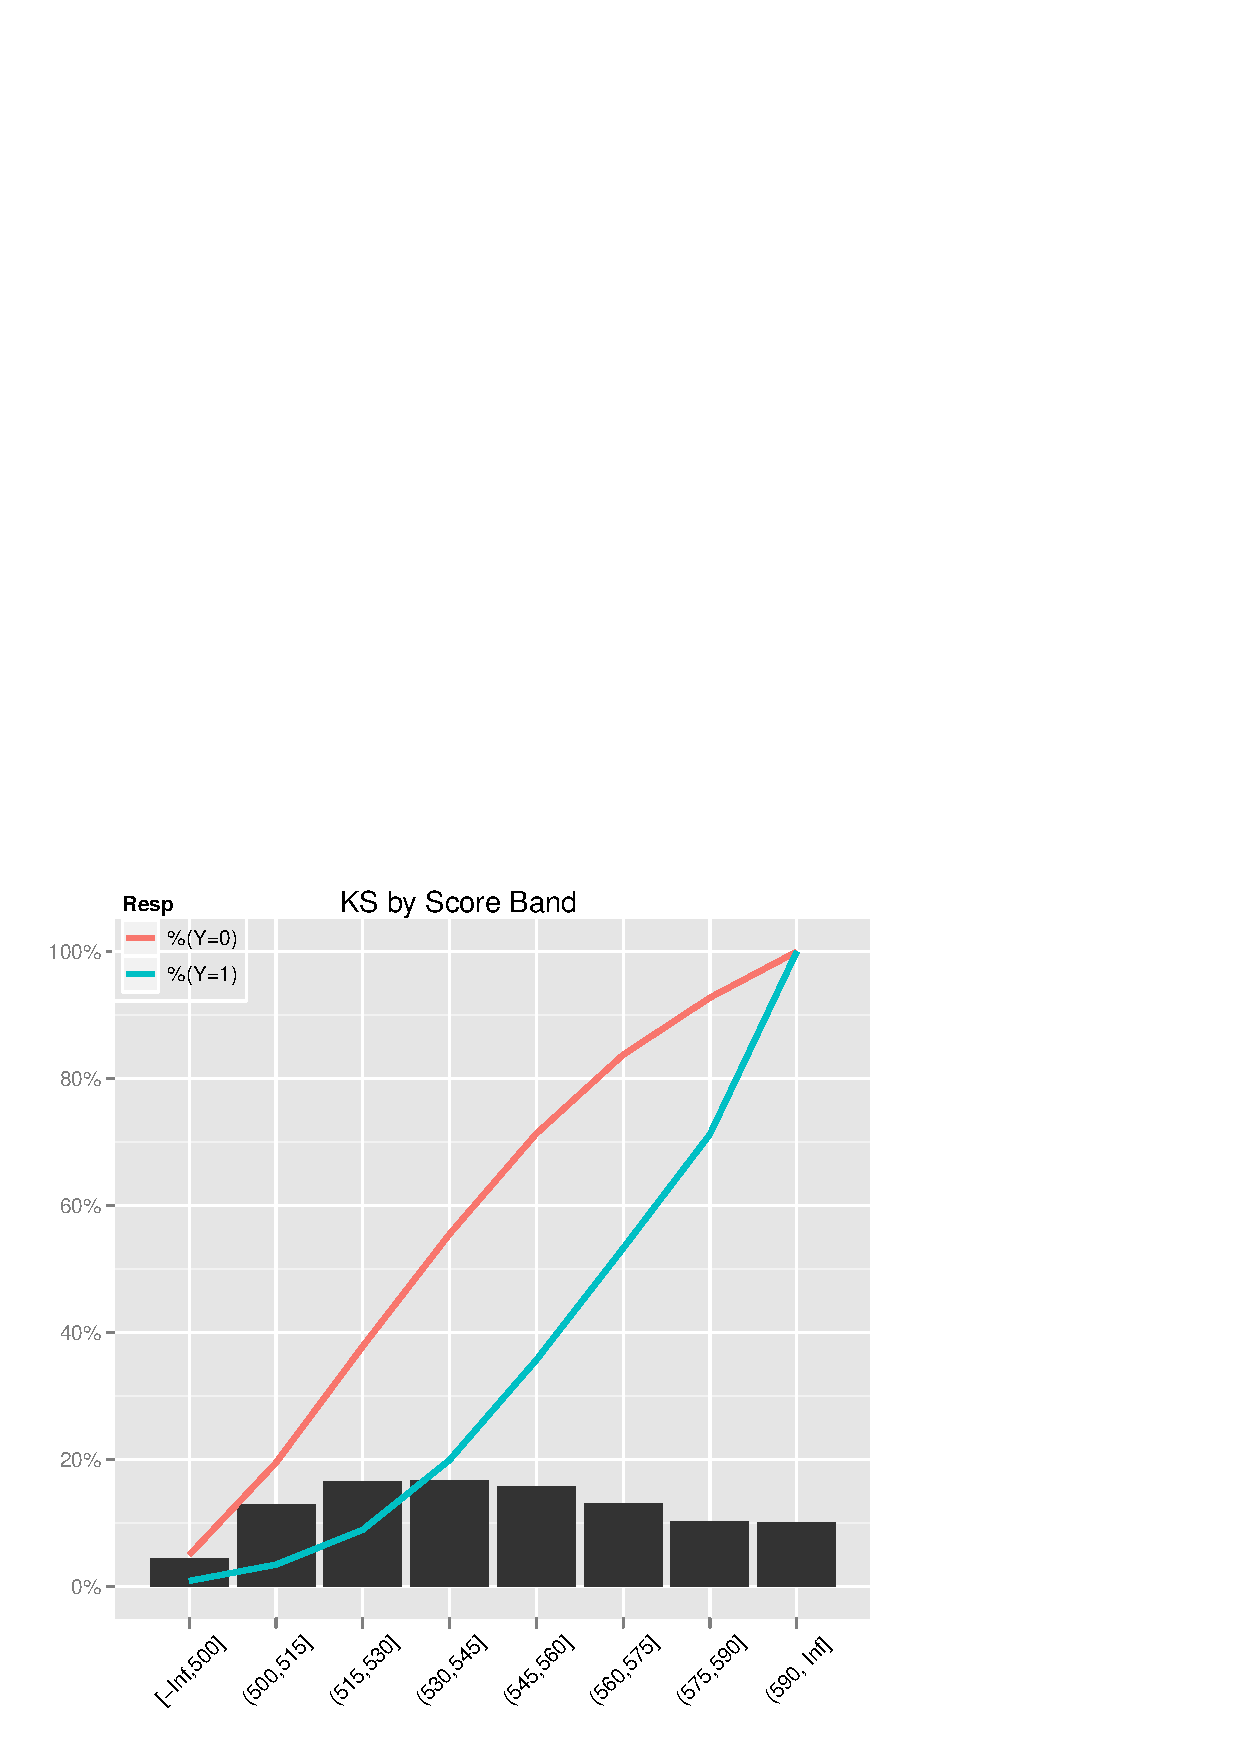
\includegraphics{ks-by-band}}
\quad
\subfigure[LogOdds Plot]{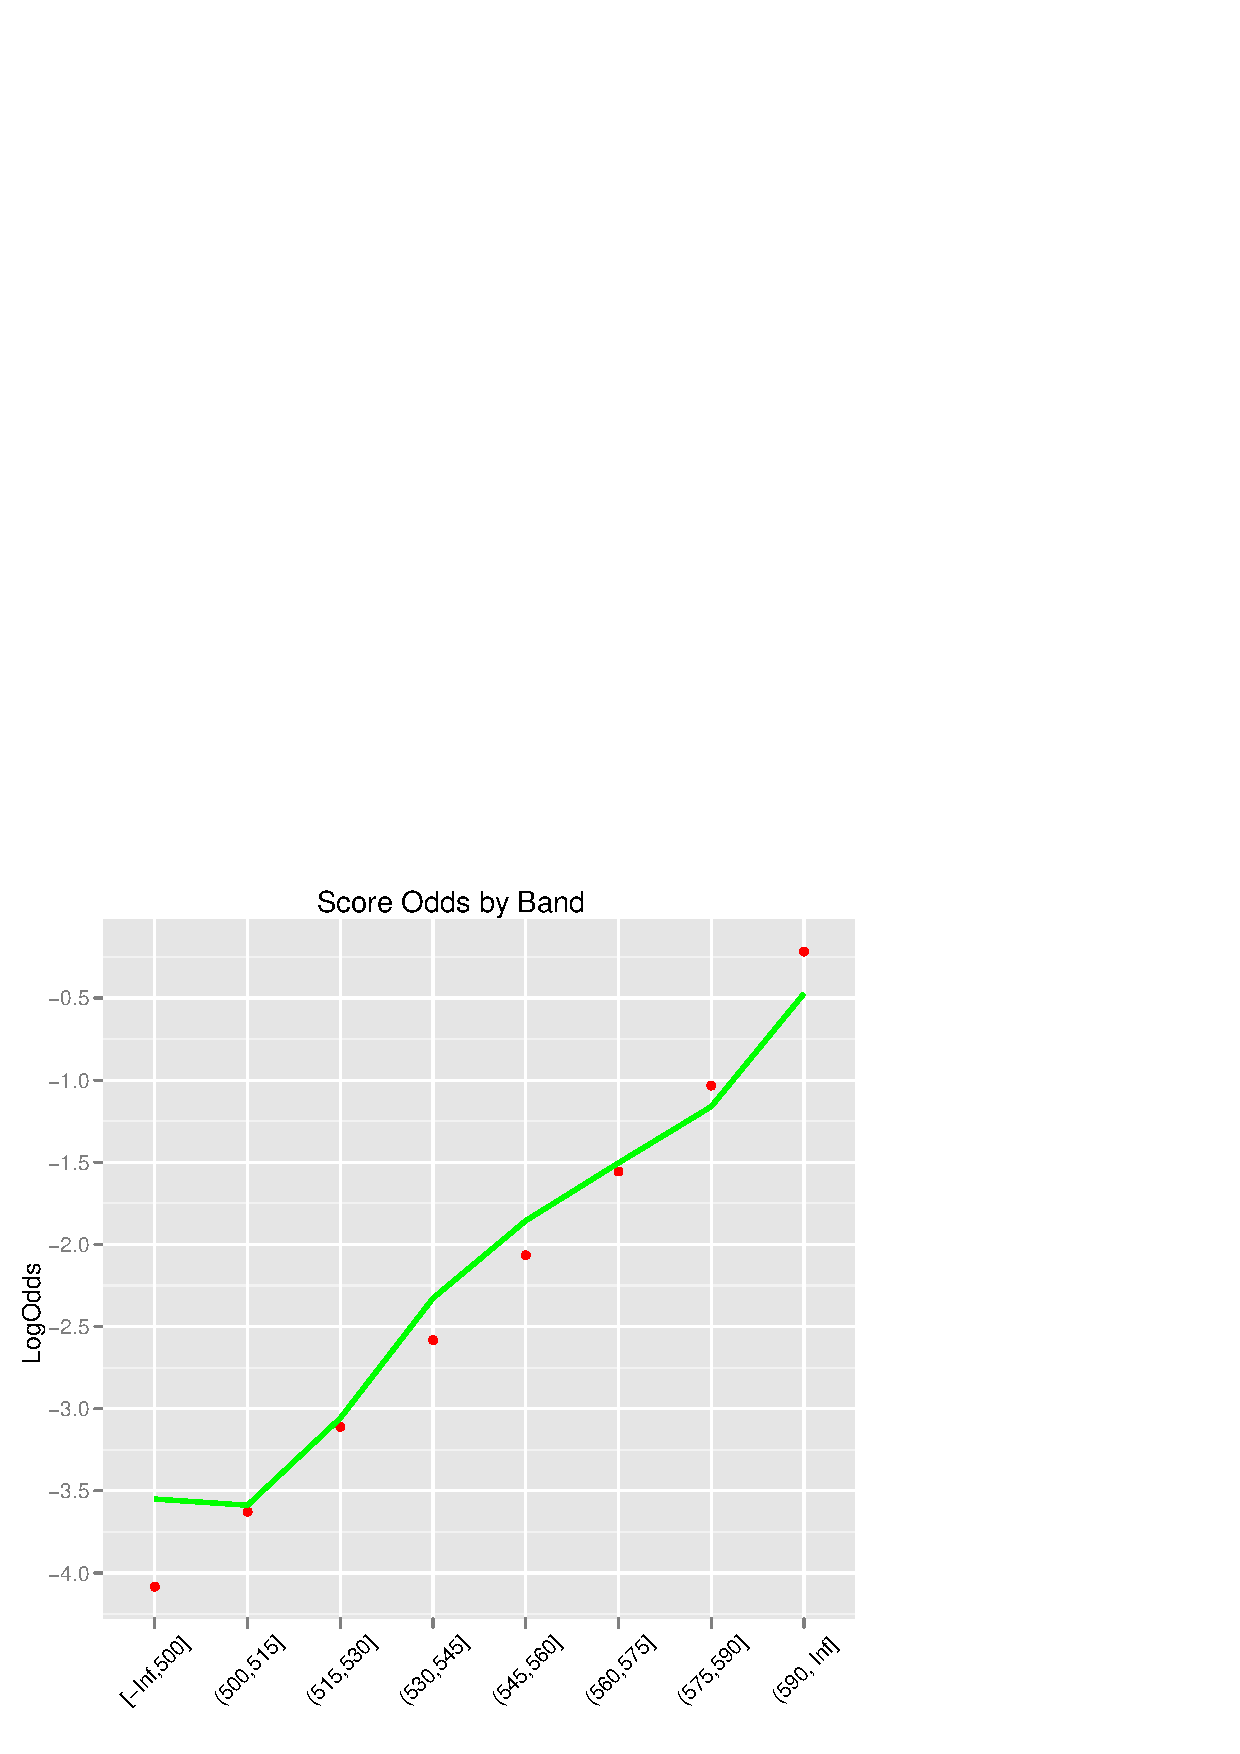
\includegraphics{score-odds-by-band}}
}
\caption{Score Band Plots}

\end{figure}



\subsection{KS table and plot by score decile} 
% \begin{center}
%<<>>=
% print(score.table.decile[, 1:7])
% @
% \end{center}
% latex table generated in R 2.11.1 by xtable 1.5-6 package
% Mon Mar 14 13:36:28 2011
\begin{table}[ht]
\begin{center}
\begin{tabular}{rrrrrrrr}
  \hline
 & Y=0 & Y=1 & Total & \%(Y=0) & \%(Y=1) & \%Total & Act.RR \\ 
  \hline
491 - 506 & 392 & 10 & 402 & 11.26 & 1.83 & 9.99 & 0.02 \\ 
  506 - 518 & 391 & 12 & 403 & 11.24 & 2.20 & 10.01 & 0.03 \\ 
  518 - 526 & 389 & 14 & 403 & 11.18 & 2.56 & 10.01 & 0.03 \\ 
  527 - 536 & 375 & 28 & 403 & 10.78 & 5.13 & 10.01 & 0.07 \\ 
  536 - 545 & 360 & 43 & 403 & 10.34 & 7.88 & 10.01 & 0.11 \\ 
  545 - 554 & 345 & 58 & 403 & 9.91 & 10.62 & 10.01 & 0.14 \\ 
  554 - 564 & 350 & 53 & 403 & 10.06 & 9.71 & 10.01 & 0.13 \\ 
  564 - 576 & 326 & 77 & 403 & 9.37 & 14.10 & 10.01 & 0.19 \\ 
  576 - 591 & 305 & 98 & 403 & 8.76 & 17.95 & 10.01 & 0.24 \\ 
  591 - 657 & 247 & 153 & 400 & 7.10 & 28.02 & 9.94 & 0.38 \\ 
   \hline
\end{tabular}
\caption{KS Table by Score Decile}
\end{center}
\end{table}



\begin{figure}
\centering
\mbox{
\subfigure[KS Plot]{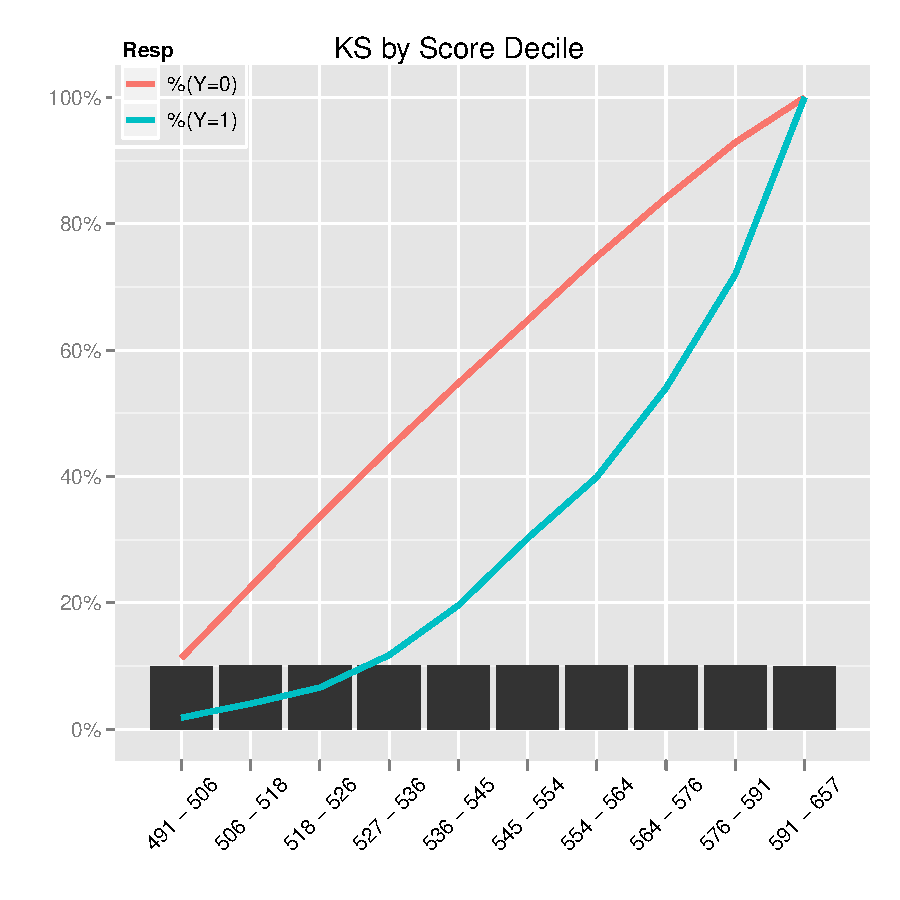
\includegraphics{ks-by-decile}}
\quad
\subfigure[LogOdds Plot]{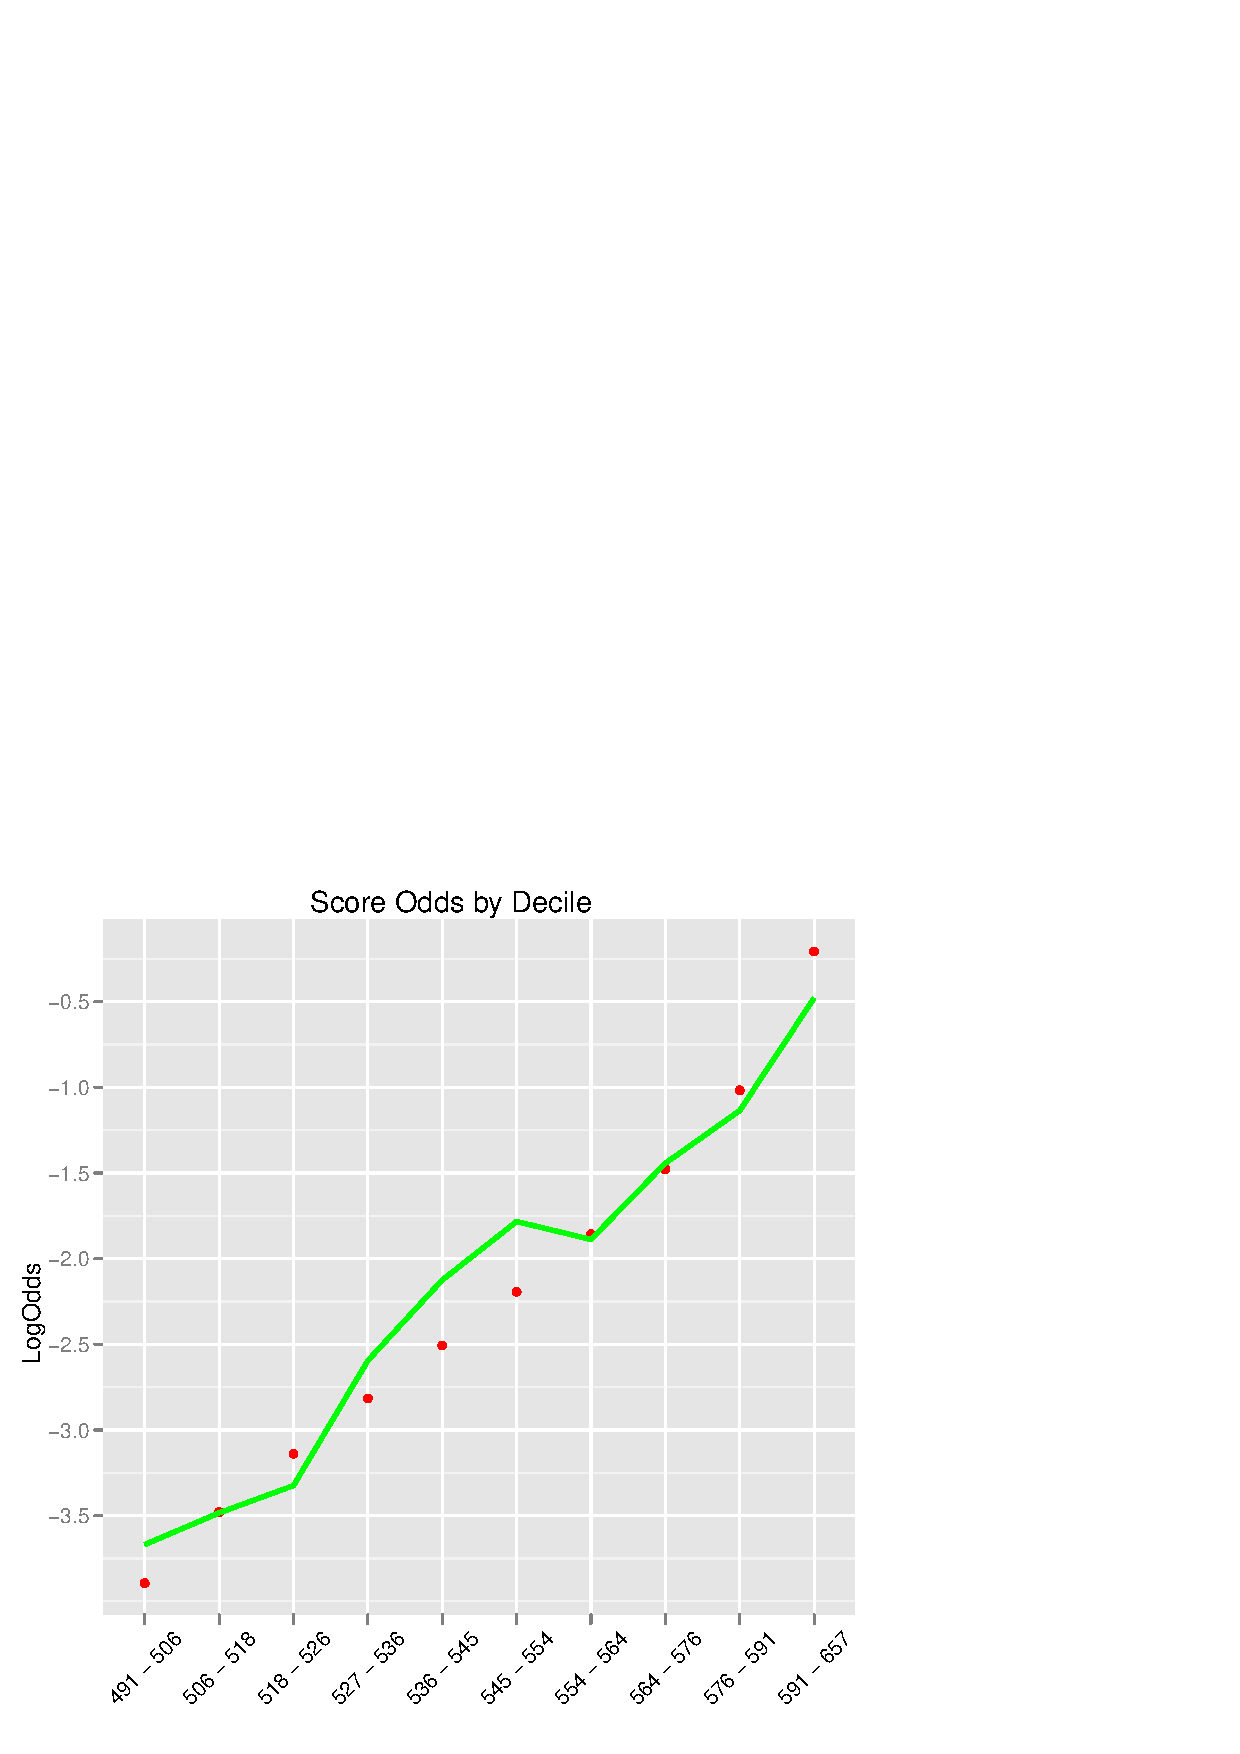
\includegraphics{score-odds-by-decile}}
}
\caption{Score Decile Plots}

\end{figure}



\end{document}


